\section{Auswertung}
\label{sec:Auswertung}

\subsection{Gedämpfte Schwingung und effektiver Dämpfungswiderstand}

Bei der Untersuchung der abklingenden Amplitude ergibt sich die
in Abbildung ... zu sehende gedämpfte Schwingung. 

%\begin{figure}
%  \centering
%  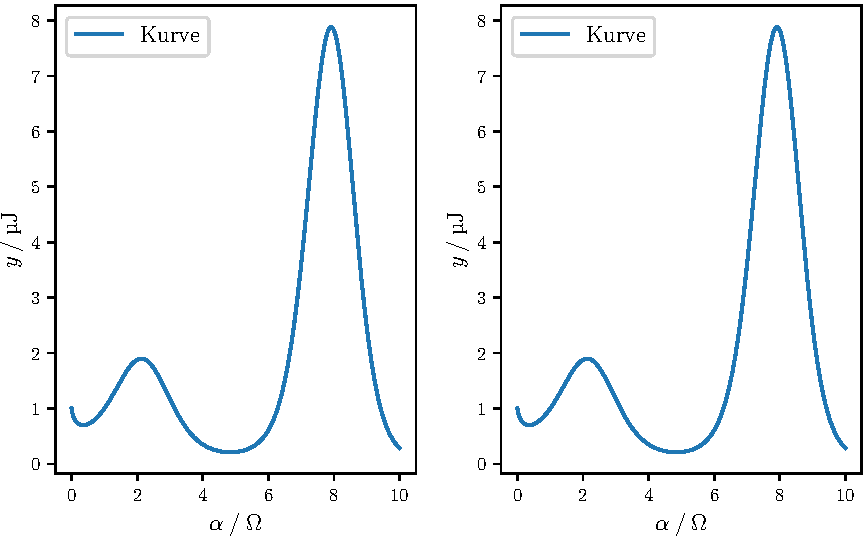
\includegraphics[scale=0.8]{plot.pdf}
%  \caption{Gedämpfte Schwingung}
%  \label{fig:gedämpft}
%\end{figure}




